%!TEX root = ../effc_top.tex

%\begin{frame}{Operations at odd primes}
%	\pause
%	Steenrod squares from derived commutativity of \textbf{binary} product.
%
%	\bigskip\pause
%	Steenrod also defined operations (for $\beta \in \{0,1\}$)
%	\[
%	\beta^{\varepsilon} P_k \colon H^\bullet(X; \Fp) \to H^\bullet(X; \Fp)
%	\]
%	from derive commutativity of higher arity product.
%
%	\bigskip\pause
%	\textcolor{pblue}{Note}: indirect definition, no explicit generalizations of cup-$i$ products.
%
%	\bigskip\pause
%	Organized by $E_\infty$-structures\pause, which have a long history:
%	\begin{itemize}
%		\item (co)homology operations, \pause
%		\item recognition of infinite loop spaces, \pause
%		\item algebraic models of the homotopy category.
%	\end{itemize}
%\end{frame}

\begin{frame}[fragile]{Operations at odd primes}
	\pause
	Squares from derived commutativity of \textbf{binary} product.

	\medskip\pause
	Steenrod also defined operations (for $\beta \in \{0,1\}$)
	\[
	\beta^{\varepsilon} P_k \colon H^\bullet(X; \Fp) \to H^\bullet(X; \Fp)
	\]
	from derive commutativity of higher arity product.

	\medskip\pause
	\textcolor{pblue}{Note}: indirect definition, no explicit generalizations of cup-$i$ structure.

	\medskip\pause
	\textcolor{pblue}{Construction (Kaufmann-Med.)} \\
	Explicit cup-$(p,i)$ products defining these operations.

	\medskip\pause
	\textcolor{pblue}{Example} \\
	Using the computer algebra system \textcolor{pblue}{\texttt{ComCH}} we have $\Delta_{3,2}[0,1,2] = $

	\begin{verbatim}
		- [0,1][0,1,2][0,1] + [0,1,2][0,2][0,1] + [0,2][0,2][0,1,2]
		- [0,1,2][0,1,2][1] - [0,2][0,1,2][1,2] + [0,1,2][1,2][1,2]
		- [0,1][1,2][0,1,2] - [0,1,2][2][0,1,2] - [0][0,1,2][0,1,2]
	\end{verbatim}
\end{frame}

\begin{frame}{A more abstract viewpoint}
	\pause
	Operads control algebraic structures, parameterizing multioperations.

	\bigskip\pause
	The operad $\mathcal{C}om$ controls commutative and associative (co)algebras.

	\bigskip\pause
	An $E_\infty$-operad is a $\Sigma$-cofibrant resolution of the terminal operad.

	\bigskip\pause
	$E_\infty$-structures have a long history:
	\smallskip\pause
	\begin{itemize}
		\item (co)homology operations,
		\item recognition of infinite loop spaces,
		\item algebraic models of the homotopy category.
	\end{itemize}

	\bigskip\pause
	The chains of spaces are $E_\infty$-coalgebras (deriving the diagonal).

	\bigskip\pause
	\textcolor{pblue}{Question}: Can this structure be concisely described?
\end{frame}

\begin{frame}{Explicit $E_\infty$-structure on (co)chains}
	\pause
	\textcolor{pblue}{Theorem (Med.)} \\
	The collection of maps $\gchains(\gsimplex^n) \to \gchains(\gsimplex^n)^{\otimes r}$ obtained from compositions of
	\begin{align*}
		\Delta &\colon \gchains(\gsimplex^n) \to \gchains(\gsimplex^n)^{\otimes 2}
		\qquad \text{(AW diagonal)} \\
		\ast &\colon \gchains(\gsimplex^n)^{\otimes 2} \to \gchains(\gsimplex^n)
		\qquad \text{(Join map)}
	\end{align*}
	defines an $E_\infty$-coalgebra on simplicial chains.

	\bigskip\pause
	\textcolor{pblue}{Example} \\
	\qquad\qquad \scalebox{0.7}{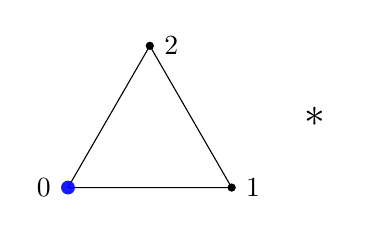
\begin{tikzpicture}[scale=.6]
\coordinate (A) at (210:2);
\coordinate (B) at (-30:2);
\coordinate (C) at (90:2);

\draw[draw=black] (A) -- (B) -- (C) -- (A);

\node[circle,fill=blue, opacity=.9, inner sep=0pt,minimum size=5pt, label=left:{0}] (a) at (A) {};
\node[circle,fill=black,inner sep=0pt,minimum size=3pt, label=right:{$1$}] (a) at (B) {};
\node[circle,fill=black,inner sep=0pt,minimum size=3pt, label=right:{$2$}] (a) at (C) {};

\node[scale=1.5] at (3.5,0.5) {$\ast$};
\end{tikzpicture}
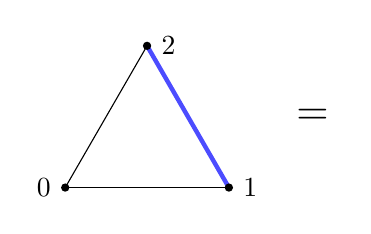
\begin{tikzpicture}[scale=.6]
\coordinate (A) at (210:2);
\coordinate (B) at (-30:2);
\coordinate (C) at (90:2);

\draw[draw=blue,  ultra thick, draw opacity=.7] (B) -- (C);
\draw[draw=black] (C) -- (A);
\draw[draw=black] (A) -- (B);

\node[circle,fill=black,inner sep=0pt,minimum size=3pt, label=left:{$0$}] (a) at (A) {};
\node[circle,fill=black,inner sep=0pt,minimum size=3pt, label=right:{$1$}] (a) at (B) {};
\node[circle,fill=black,inner sep=0pt,minimum size=3pt, label=right:{$2$}] (a) at (C) {};

\node[scale=1.5] at (3.5,.5) {=};
\end{tikzpicture}
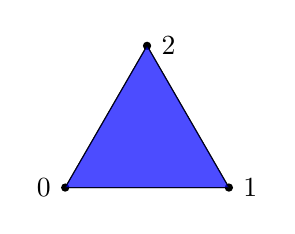
\begin{tikzpicture}[scale=.6]
\coordinate (A) at (210:2);
\coordinate (B) at (-30:2);
\coordinate (C) at (90:2);

\draw[draw=black] (A) -- (B) -- (C) -- (A);

\node[circle,fill=black,inner sep=0pt,minimum size=3pt, label=left:{$0$}] (a) at (A) {};
\node[circle,fill=black,inner sep=0pt,minimum size=3pt, label=right:{$1$}] (a) at (B) {};
\node[circle,fill=black,inner sep=0pt,minimum size=3pt, label=right:{$2$}] (a) at (C) {};

\draw[draw, fill=blue, opacity=.7] (A) -- (B) -- (C) -- (A);
\end{tikzpicture}}

	\bigskip\pause
	\textcolor{pblue}{Other versions} \\
	Cubical (Kaufmann--Med.) \\
	Multisimplicial (Med.--Pizzi--Salvatore).
\end{frame}

\begin{frame}{A finitely presented $E_\infty$-prop}
	\pause Consider the (algebraic) prop $\cM$ generated by
%	\vskip-5pt
	\[
	\begin{tikzpicture}[scale=.4]
		\draw (0,.5)--(0,-.75);
		\node[scale=.5] at (0,.75){1};
		\fill (0,-.65) circle (3pt);
	\end{tikzpicture}
	\qquad
	\begin{tikzpicture}[scale=.4]
		\draw (0,0)--(0,.75);
		\draw (0,0)--(.5,-.5);
		\draw (0,0)--(-.5,-.5);
		\node[scale=.5] at (-.5,-.75){1};
		\node[scale=.5] at (.5,-.75){2};
	\end{tikzpicture}
	\qquad
	\begin{tikzpicture}[scale=.4]
		\draw (0,0)--(0,-.75);
		\draw (0,0)--(.5,.5);
		\draw (0,0)--(-.5,.5);
		\node[scale=.5] at (-.5,.75){1};
		\node[scale=.5] at (.5,.75){2};
	\end{tikzpicture}
	\vspace*{-2pt}
	\]
	in degrees $0, 0$ \& $1$ with non-zero boundary
	\[
	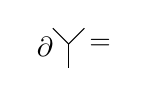
\begin{tikzpicture}[scale=.4]
		\node[scale=1] at (-.75,-.1){$\partial$};
		\draw (0,0)--(0,-.75);
		\draw (0,0)--(.5,.5);
		\draw (0,0)--(-.5,.5);
		\node[scale=1] at (1,0){$=$};
	\end{tikzpicture}
	\begin{tikzpicture}[scale=.4]
		\draw (0,.5)--(0,-.75);
		\fill (0,-.65) circle (3pt);
		\draw (.5,.5)--(.5,-.75);
		\node[scale=1] at (1.1,0){$-$};
	\end{tikzpicture}
	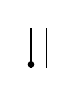
\begin{tikzpicture}[scale=.4]
		\draw (0,.5)--(0,-.75);
		\fill (0,-.65) circle (3pt);
		\draw (.5,.5)--(.5,-.75);
	\end{tikzpicture}
	\]
	\vskip-5pt
	and relators
	\[
	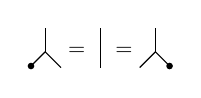
\begin{tikzpicture}[scale=.4]
		\draw (0,0)--(0,.75);
		\draw (0,0)--(.5,-.5);
		\draw (0,0)--(-.5,-.5);
		\fill (-.45,-.45) circle (3pt);
		\node[scale=.8] at (1,0){$=$};
		\draw (1.75,.75)--(1.75,-.5);
		\node[scale=.8] at (2.5,0){$=$};
		\draw (3.5,0)--(3.5,.75);
		\draw (3.5,0)--(4,-.5);
		\draw (3.5,0)--(3,-.5);
		\fill (3.95,-.45) circle (3pt);
	\end{tikzpicture}
	\quad\qquad
	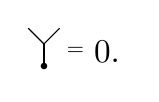
\begin{tikzpicture}[scale=.4]
		\draw (0,0)--(0,-.75);
		\draw (0,0)--(.5,.5);
		\draw (0,0)--(-.5,.5);
		\fill (0,-.7) circle (3pt);
		\node[scale=.8] at (1,-.25){$=$};
		\node[scale=1.2] at (2,-.25){$0.$};
	\end{tikzpicture}
	\]

	\medskip\pause
	\textcolor{pblue}{Theorem (Med.)} \\
	$\forget(\cM) \defeq \{\cM(1,r)\}_{r \geq 1}$ is a (cofibrant and Hopf) $E_\infty$-operad.
\end{frame}

%\begin{frame}{Two $E_\infty$-bialgebra models for loop spaces}
%	\pause
%	Based space $(X,x)$ $\rightarrow$ ``topological monoid'' $\Omega_x X$
%
%	\medskip\pause
%	Cubical singular chains define $\rS^{\square}(\Omega_x X)$ a monoid in $\mathsf{Ch}$.
%
%	\medskip\pause
%	Adams cobar construction applied to based singular chains $\mathbb{\Omega} \rS^{\triangle}(X, x)$:
%
%\end{frame}

\begin{frame}[fragile]{Two $E_\infty$-bialgebra models for loop spaces}
	\pause
	\textcolor{pblue}{Construction (Adams)}
	\vspace*{-1pt}
	\begin{center}
		Based space $(X,x)$ \\ \pause
%		$\Downarrow$ \\
%		``Topological monoid'' $\Omega_x X$ \\ \pause
		$\Downarrow$ \\
		Two algebras
		and a q-iso of algebras: \\
		\medskip
		$\mathbb{\Omega} \rS^{\triangle}(X, x)$
		$\xra{\quad \theta_X \quad }$
		$\rS^{\square}(\Omega_x X)$
	\end{center}

	\begin{minipage}{.45\textwidth}
		\begin{flushright}
			Cobar const. on based \\
			simplicial sing. chains
		\end{flushright}
	\end{minipage}
	\hspace*{.9cm}
	\begin{minipage}{.4\textwidth}
		Cubical sing. chains \\
		on based loop space
	\end{minipage}

	\bigskip\smallskip\pause
	\textcolor{pblue}{Theorem (Baues)} \\
	$\theta_X$ is a map of bialgebras.

	\bigskip\pause
	\textcolor{pblue}{Theorem (Med.--Rivera)} \\
	$\theta_X$ is a map of $E_\infty$-bialgebras.
\end{frame}

%\begin{frame}[fragile]{Cup-$(p,i)$ products}
%
%	\vskip-5pt\pause
%
%	\begin{block}{Construction (Kaufmann-Med.)}
%		Explicit cup-$(p,i)$ coproducts defining \textcolor{pblue}{operations} on $H^\bullet(-; \Fp)$.
%	\end{block}
%
%	\pause
%
%	\begin{block}{Implementation (Med.)}
%		In the computer algebra system \textcolor{pblue}{\texttt{ComCH}}.
%	\end{block}
%
%	\pause
%
%	For example, $\Delta_{3,2}[0,1,2]$ is equal to
%
%	\begin{verbatim}
%		- [0,1][0,1,2][0,1] + [0,1,2][0,2][0,1] + [0,2][0,2][0,1,2]
%		- [0,1,2][0,1,2][1] - [0,2][0,1,2][1,2] + [0,1,2][1,2][1,2]
%		- [0,1][1,2][0,1,2] - [0,1,2][2][0,1,2] - [0][0,1,2][0,1,2]
%	\end{verbatim}
%
%	\pause
%
%	\textcolor{pblue}{Future directions:} (from the even to odd primes)
%
%	\pause
%	\begin{enumerate}
%		\item Faster implementations for use in TDA. \pause \\
%		\item Relation to higher category theory. \pause \\
%		\item Connections to convex geometry. \pause \\
%		\item Cartan and Adem coboundaries. \pause \\
%		\item Where are these used in physics?
%	\end{enumerate}
%\end{frame}